\documentclass[tikz,border=15pt]{standalone}
\usepackage{pgfplots}
\usetikzlibrary{patterns, arrows.meta}
\pgfplotsset{compat=1.18}

\begin{document}
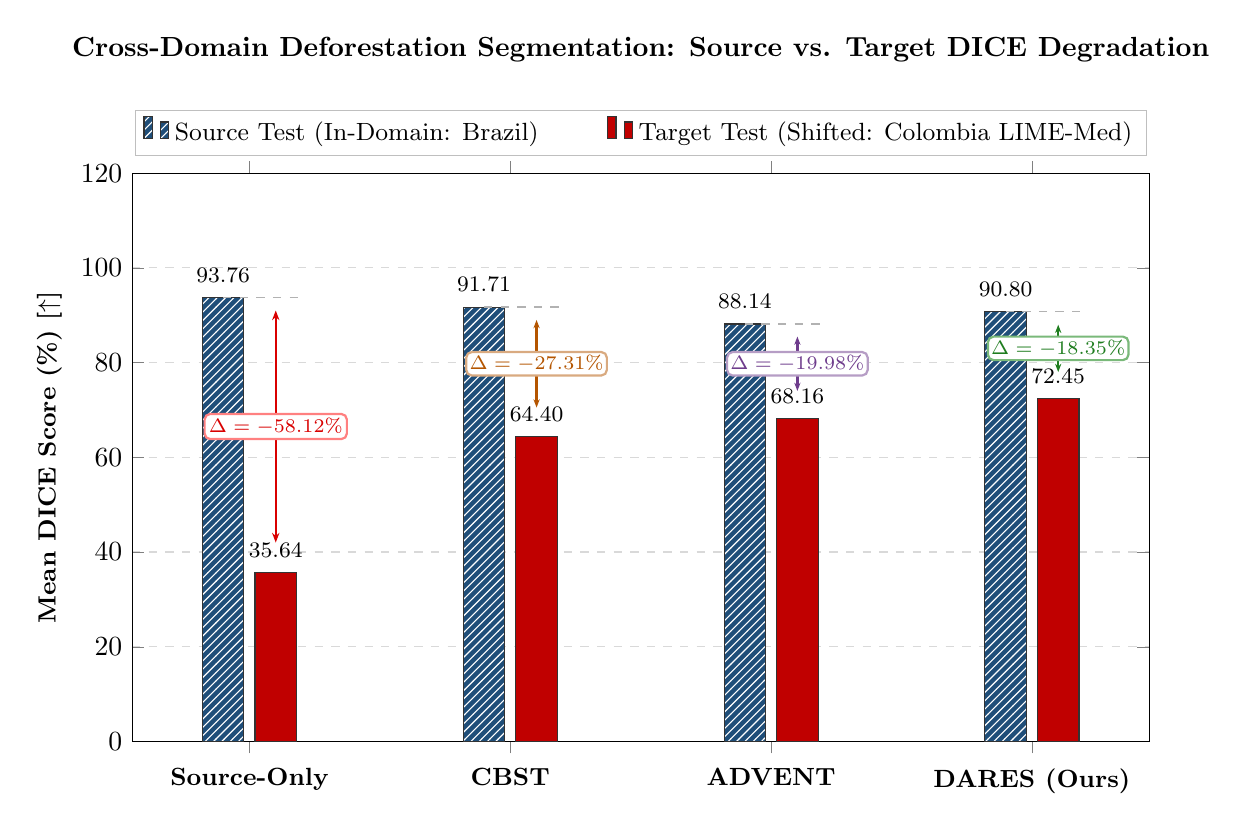
\begin{tikzpicture}
    % Color palette for publication
    \definecolor{sourcecolor}{RGB}{31, 78, 121}   % Deep Navy Blue
    \definecolor{targetcolor}{RGB}{192, 0, 0}     % Academic Crimson Red
    \definecolor{cbstcolor}{RGB}{180, 85, 0}      % Amber / Rust
    \definecolor{adventcolor}{RGB}{110, 60, 140}  % Purple / Slate
    \definecolor{darescolor}{RGB}{34, 139, 34}    % Forest Green (Ours)

    \begin{axis}[
        ybar=4pt,
        bar width=15pt,
        width=14.5cm,
        height=8.8cm,
        ymin=0,
        ymax=120,
        enlarge x limits=0.15,
        ylabel={\textbf{Mean DICE Score (\%) [$\uparrow$]}},
        ylabel style={font=\small},
        symbolic x coords={Source-Only, CBST, ADVENT, DARES},
        xtick=data,
        xticklabels={Source-Only, CBST, ADVENT, {DARES (Ours)}},
        x tick label style={font=\small\bfseries, yshift=-2pt},
        ymajorgrids=true,
        grid style={dashed, gray!30},
        % Formato estricto a 2 decimales
        nodes near coords,
        every node near coord/.append style={
            font=\footnotesize\bfseries,
            yshift=2pt,
            /pgf/number format/fixed,
            /pgf/number format/precision=2,
            /pgf/number format/fixed zerofill
        },
        % Leyenda desacoplada del título
        legend style={
            at={(0.5, 1.03)},
            anchor=south,
            legend columns=2,
            font=\small,
            draw=gray!50,
            fill=white,
            /tikz/every even column/.append style={column sep=0.8cm}
        },
        title style={font=\bfseries, at={(0.5, 1.15)}, anchor=south},
        title={Cross-Domain Deforestation Segmentation: Source vs. Target DICE Degradation}
    ]

        % 1. SOURCE TEST (In-Domain Reference)
        \addplot[
            fill=sourcecolor,
            draw=black!80,
            postaction={pattern=north east lines, pattern color=white!40}
        ] coordinates {
            (Source-Only, 93.76)
            (CBST, 91.71)
            (ADVENT, 88.14)
            (DARES, 90.80)
        };
        \addlegendentry{Source Test (In-Domain: Brazil)}

        % 2. TARGET TEST (Cross-Domain Covariate Shift)
        \addplot[
            fill=targetcolor,
            draw=black!80
        ] coordinates {
            (Source-Only, 35.64)
            (CBST, 64.40)
            (ADVENT, 68.16)
            (DARES, 72.45)
        };
        \addlegendentry{Target Test (Shifted: Colombia LIME-Med)}

        % -------------------------------------------------------------
        % 1. SOURCE-ONLY DELTA (Gap: 93.76 -> 35.64 = -58.12%)
        % -------------------------------------------------------------
        \draw[dashed, gray!60, line width=0.5pt] 
            ([xshift=-9.5pt]axis cs:Source-Only, 93.76) -- ([xshift=18pt]axis cs:Source-Only, 93.76);
        \draw[{Stealth[length=3.5pt]}-{Stealth[length=3.5pt]}, thick, red!85!black] 
            ([xshift=9.5pt]axis cs:Source-Only, 42) -- ([xshift=9.5pt]axis cs:Source-Only, 91)
            node[midway, fill=white, inner sep=1.5pt, rounded corners=2pt, draw=red!50, font=\scriptsize\bfseries, text=red!85!black] 
            {$\Delta = -58.12\%$};

        % -------------------------------------------------------------
        % 2. CBST DELTA (Gap: 91.71 -> 64.40 = -27.31%)
        % -------------------------------------------------------------
        \draw[dashed, gray!60, line width=0.5pt] 
            ([xshift=-9.5pt]axis cs:CBST, 91.71) -- ([xshift=18pt]axis cs:CBST, 91.71);
        \draw[{Stealth[length=3pt]}-{Stealth[length=3pt]}, thick, cbstcolor] 
            ([xshift=9.5pt]axis cs:CBST, 70.5) -- ([xshift=9.5pt]axis cs:CBST, 89)
            node[midway, fill=white, inner sep=1.2pt, rounded corners=2pt, draw=cbstcolor!50, font=\scriptsize\bfseries, text=cbstcolor] 
            {$\Delta = -27.31\%$};

        % -------------------------------------------------------------
        % 3. ADVENT DELTA (Gap: 88.14 -> 68.16 = -19.98%)
        % -------------------------------------------------------------
        \draw[dashed, gray!60, line width=0.5pt] 
            ([xshift=-9.5pt]axis cs:ADVENT, 88.14) -- ([xshift=18pt]axis cs:ADVENT, 88.14);
        \draw[{Stealth[length=3pt]}-{Stealth[length=3pt]}, thick, adventcolor] 
            ([xshift=9.5pt]axis cs:ADVENT, 74) -- ([xshift=9.5pt]axis cs:ADVENT, 85.5)
            node[midway, fill=white, inner sep=1.2pt, rounded corners=2pt, draw=adventcolor!50, font=\scriptsize\bfseries, text=adventcolor] 
            {$\Delta = -19.98\%$};

        % -------------------------------------------------------------
        % 4. DARES (OURS) DELTA (Gap: 90.80 -> 72.45 = -18.35%)
        % -------------------------------------------------------------
        \draw[dashed, gray!60, line width=0.5pt] 
            ([xshift=-9.5pt]axis cs:DARES, 90.80) -- ([xshift=18pt]axis cs:DARES, 90.80);
        \draw[{Stealth[length=3pt]}-{Stealth[length=3pt]}, thick, darescolor!90!black] 
            ([xshift=9.5pt]axis cs:DARES, 78) -- ([xshift=9.5pt]axis cs:DARES, 88)
            node[midway, fill=white, inner sep=1.2pt, rounded corners=2pt, draw=darescolor!60, font=\scriptsize\bfseries, text=darescolor!90!black] 
            {$\Delta = -18.35\%$};

    \end{axis}
\end{tikzpicture}
\end{document}